\section*{Autores}

\begin{wrapfigure}{l}{0.3\linewidth}
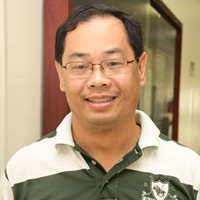
\includegraphics[width=\linewidth]{figuras/autor1.jpg}
\end{wrapfigure}

 \textbf{Carlos Alberto Ynoguti} Possui graduação em Engenharia Elétrica pela Universidade de São Paulo(1991), mestrado em Engenharia Elétrica pela Universidade de São Paulo(1995), doutorado em Engenharia Elétrica pela Universidade Estadual de Campinas(2000) e pós-doutorado pela Universidade Estadual de Campinas(2001). Atualmente é Professor Adjunto do Instituto Nacional de Telecomunicações e Membro de corpo editorial da Telecomunicações (Santa Rita do Sapucaí) (1516-2338). Tem experiência na área de Engenharia Elétrica, com ênfase em Telecomunicações. Atuando principalmente nos seguintes temas:processamento digital de sinais, processamento de voz, reconhecimento de fala. 

\begin{wrapfigure}{l}{0.3\linewidth}
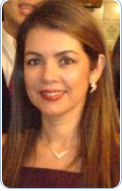
\includegraphics[width=\linewidth]{figuras/autor2.png}  
\end{wrapfigure}

   \textbf{Rosanna Mara Rocha Silveira} Possui graduação (1985) em Ciência da Computação pela UFMG (Universidade Federal de Minas Gerais) e mestrado (2003) em Engenharia Elétrica pela UNICAMP (Universidade Estadual de Campinas). Atualmente é professora adjunta da Fundação Instituto Nacional de Telecomunicações (INATEL). Na área de Engenharia tem atuação nas seguintes subáreas: algoritmos, estruturas de dados, banco de dados, modelagem e simulação, simulação de evento discreto, métodos numéricos, redes de comunicação sem fio, múltiplo acesso, análise e desempenho de redes de comunicação, processamento de sinais, transformadas wavelets e compressão de sinais.

\begin{wrapfigure}{l}{0.3\linewidth}
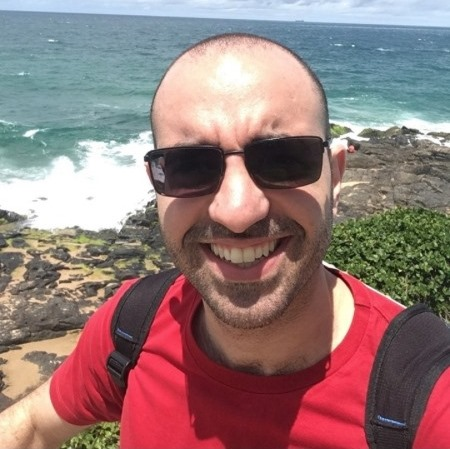
\includegraphics[width=\linewidth]{figuras/autor3.png}
\end{wrapfigure}

    \textbf{Phyllipe Lima} é Doutor em Computação Aplicada (2021) pelo INPE - Instituto Nacional de Pesquisas Espaciais, na área de Engenharia de Software realizando estudos sobre metadados através da análise estática de código fonte e MSR (Mining Software Repositories). Mestre em Ciência da Computação(2016) pela UNIFEI - Universidade Federal de Itajubá. Engenheiro de Telecomunicações(2011) pelo INATEL - Instituto Nacional de Telecomunicações.  Técnico em Telecomunicações(2006) pela Escola Técnica de Eletrônica - ETE "FMC". É professor auxiliar do INATEL, atuando nos cursos de Engenharia da Computação e Engenharia de Software. Tem interesse nas áreas de Engenharia de Software Empírica, Desenvolvimento de Jogos e Computação Gráfica.


   
   
   
   
   
